\textbf{Agenda}

Pada chapter ini kita akan membahas tentang beberapa class khusus yang
ada pada Qt Core Module yang dapat digunakan untuk melengkapi library
standar C++ yang sebelumnya sudah kita gunakan. Adapun beberapa topik
yang akan kita bahas pada chapter ini adalah.

\minitoc

\section{Qt Library}\label{qt-library-1}

Qt SDK menyediakan beberapa class library yang dapat anda gunakan untuk
mempercepat pembuatan program, misalnya library untuk membuat GUI
(Graphical User Interface), network programming, dan library untuk
bekerja dengan XML. Beberapa class library yang disediakan oleh Qt dapat
dilihat pada gambar \ref{fig:qt-library}.

\begin{figure}[htbp]
\centering
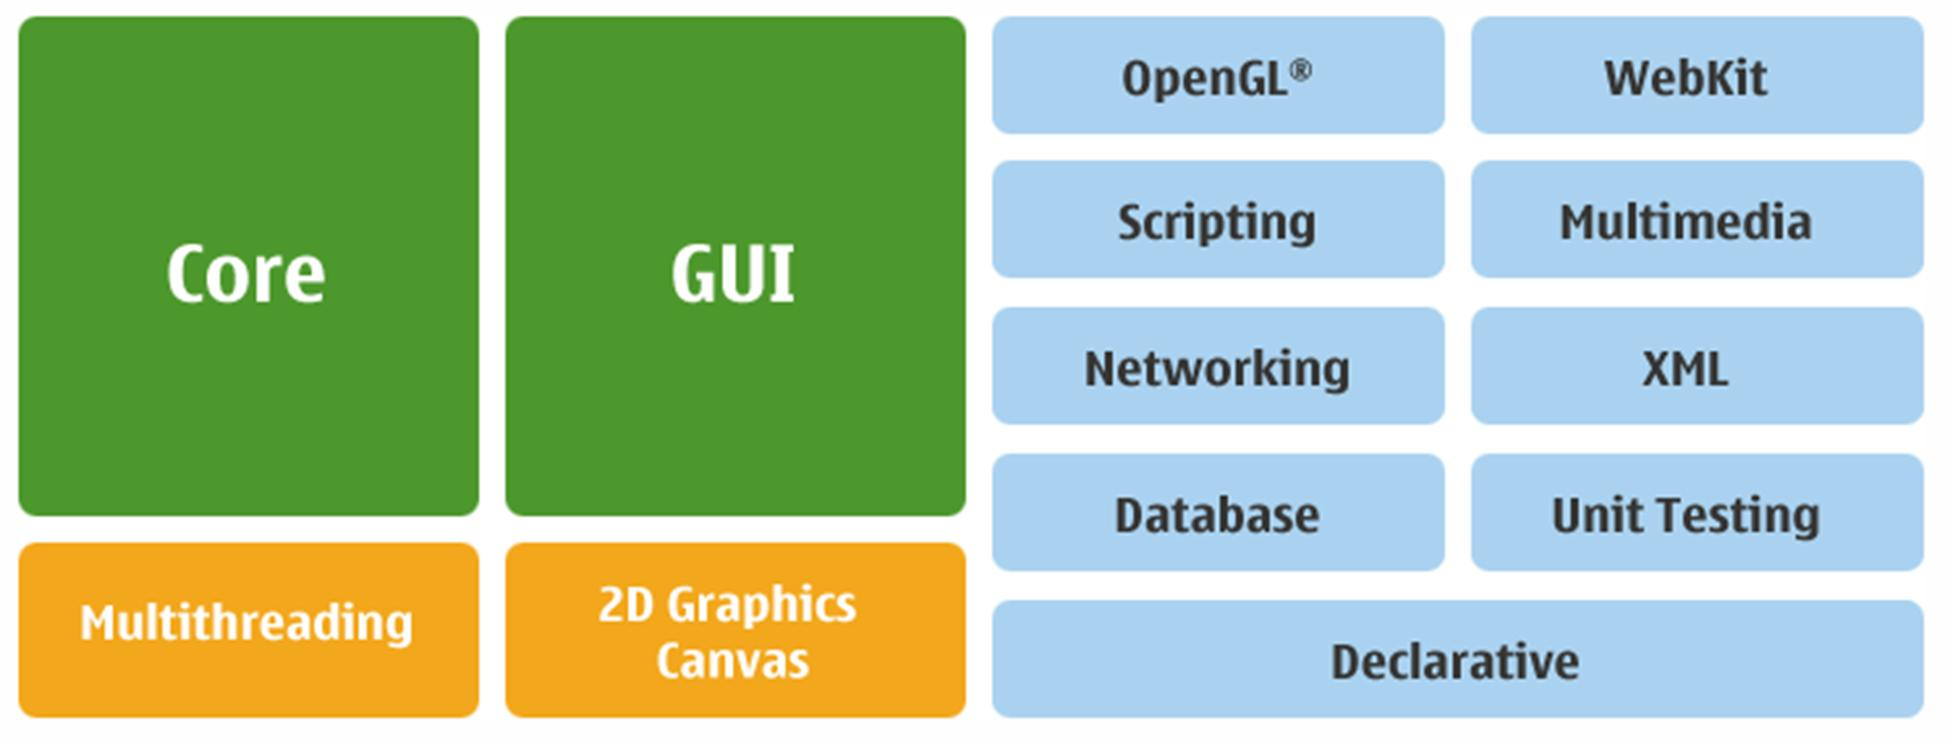
\includegraphics[width=0.9\linewidth]{images/qt-library}
\caption{Class libray yang di sediakan oleh Qt}
\label{fig:qt-library}
\end{figure}


Pada chapter ini kita akan membahas beberapa class dalam Qt Core Module
yang sering digunakan seperti QObject, QString dan QStringList.

Qt Core Module adalah library yang dibutuhkan oleh setiap aplikasi Qt.
Qt Core Module sendiri dapat berisi :

\begin{itemize}

\item
  Basic Data Type seperti QString dan QByteArray.
\item
  Basic Data Structure seperti QList, QVector, dan QHash.
\item
  Input/Output class seperti QIODevice, QTextStream, dan QFile.
\item
  Class untuk pemrograman multithread seperti Qthread.
\item
  Class Object dan QCoreApplication (base class dari QApplication).
\end{itemize}

\section{Menurunkan objek dari class QObject}\label{menurunkan-objek-dari-class-qobject}

QObject class merupakan base class dari sebagian class yang ada di Qt
library. Dengan menurunkan class dari QObject maka anda dapat
menggunakan fitur automatic memory management dan mekanisme signal/slot
yang disediakan oleh Qt.

Beberapa class pada Qt yang diturunkan dari class QObject diantaranya
QWidget, QLayout, dan QThread. Ada juga class yang tidak diturunkan dari
class QObject seperti QString dan QColor.

Gambar \ref{fig:qobjek} menunjukan contoh beberapa class yang diturunkan dari
QObject.

\begin{figure}
\centering
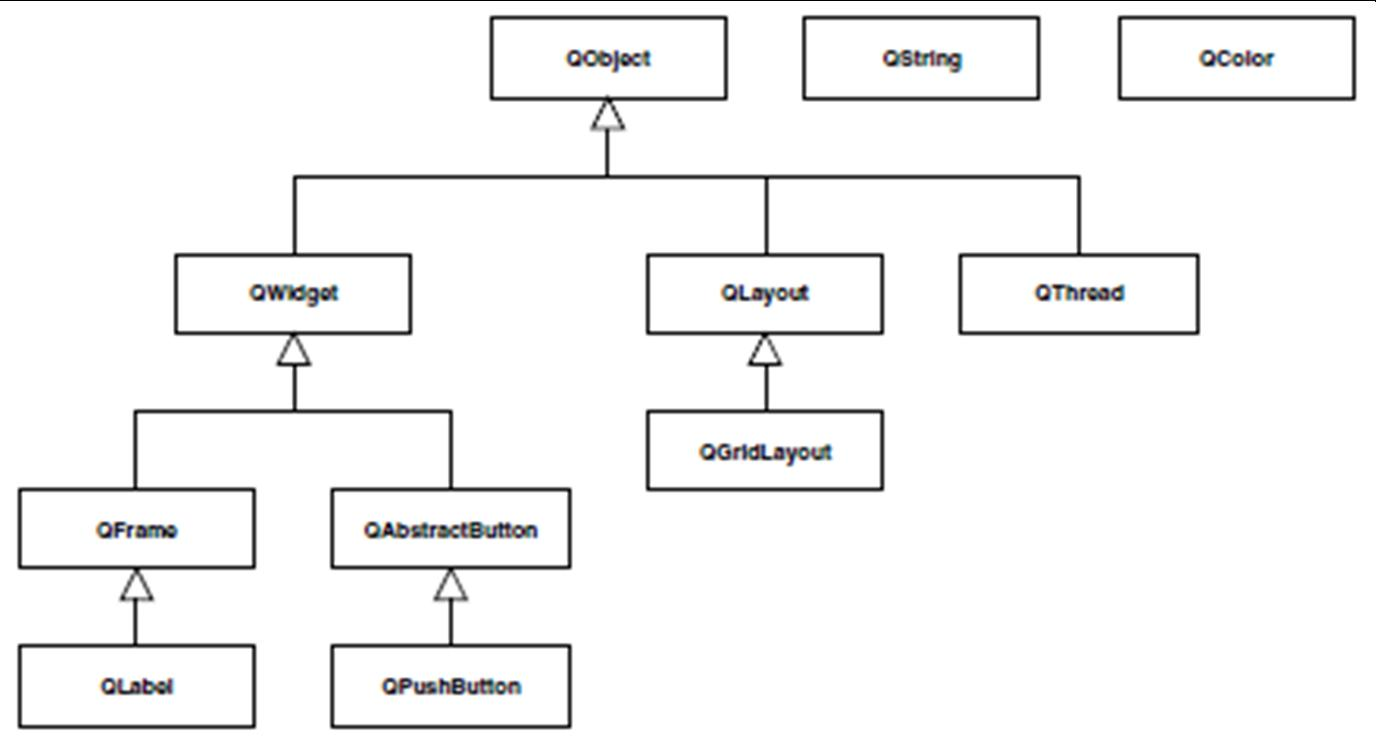
\includegraphics[width=0.9\linewidth]{images/Qobjek}
\caption{Turunan objek dari class QObject}
\label{fig:qobjek}
\end{figure}


\section{Automatic Memory Management dengan
QObject}\label{automatic-memory-management-dengan-qobject}

Dengan menurunkan class dari QObject anda dapat melakukan automatic
memory management pada program anda, sehingga kemungkinan terjadi memory
leak dapat dihindari. Pada contoh dibawah ini kita akan membuat dua
program yang berbeda, program pertama tidak menggunakan QObject dan
program kedua menggunakan QObject.

\subsubsection*{Contoh  Alokasi memory dinamis tanpa QObject.}

\begin{enumerate}

\item
  Buka Qt Creator dan buat project Qt Console Application baru dengan
  nama Contoh \ref{contoh-11.1}, kemudian tulis kode berikut.

\begin{lstlisting}[language=c++, caption= Alokasi memory dinamis tanpa QObject, label=contoh-11.1]
#include <QtCore/QCoreApplication>
#include <iostream>
#include <string>
using namespace std;
class Mahasiswa
{
public:
Mahasiswa(const string &nim);
~Mahasiswa();
const string &nim() const;
void setNim(const string &nim);
int getNimLength() const;
private:
string _nim;
};
Mahasiswa::Mahasiswa(const string &nim)
{
_nim = nim;
}
Mahasiswa::~Mahasiswa()
{
cout << "destroy object" << endl;
}
const string &Mahasiswa::nim() const
{
return _nim;
}
void Mahasiswa::setNim(const string &nim)
{
_nim = nim;
}
int Mahasiswa::getNimLength() const
{
return _nim.length();
}
int main(int argc, char *argv[])
{
QCoreApplication a(argc, argv);
Mahasiswa *objMhs1,*objMhs2,*objMhs3;
objMhs1 = new Mahasiswa("22002321");
objMhs2 = new Mahasiswa("22002322");
objMhs3 = new Mahasiswa("22002323");
cout << objMhs1->nim() << " : " << objMhs1->getNimLength() << " kar" << endl;
objMhs1->setNim(objMhs2->nim());
objMhs2->setNim(objMhs3->nim());
cout << objMhs1->nim() << " : " << objMhs1->getNimLength() << " kar" << endl;
cout << objMhs2->nim() << " : " << objMhs2->getNimLength() << " kar" << endl;
cout << objMhs3->nim() << " : " << objMhs3->getNimLength() << " kar" << endl;
delete objMhs1;
delete objMhs2;
delete objMhs3;
return a.exec();
}
\end{lstlisting}
\item
  Kemudian jalankan kode diatas dengan menekan tombol Ctrl+R, maka akan
  ditampilkan output sebagai berikut.
  
  \begin{lcverbatim}
22002321 : 8 kar
22002322 : 8 kar
22002323 : 8 kar
22002323 : 8 kar
destroy object
destroy object
destroy object
  \end{lcverbatim}
\end{enumerate}

\textbf{Keterangan:}

\begin{itemize}

\item
  Class Mahasiswa yang kita buat diatas tidak diturunkan dari class
  QObject, sehingga kita harus menghapus memory di heap yang sudah tidak
  digunakan kembali secara manual untuk menghindari memory leak.
\item
  Penanganan secara manual menuntut programmer untuk lebih teliti dan
  akan menyulitkan bila membangun aplikasi yang kompleks dan memiliki
  banyak objek.
\end{itemize}

\subsubsection*{Contoh  Alokasi memory dinamis dengan QObject.}

\begin{enumerate}

\item
  Buka Qt Creator dan buat project Qt Console Application baru dengan
  nama Contoh \ref{contoh-11.2}, kemudian tulis kode berikut.

\begin{lstlisting}[language=c++, caption=Alokasi memory dinamis dengan QObject, label=contoh-11.2]
#include <QtCore/QCoreApplication>
#include <QObject>
#include <QDebug>
using namespace std;
class Mahasiswa : QObject
{
public:
Mahasiswa(const QString &nim,QObject *parent=0);
const QString &nim() const;
void setNim(const QString &nim);
int getNimLength() const;
private:
QString _nim;
};
Mahasiswa::Mahasiswa(const QString &nim, QObject *parent)
{
_nim = nim;
}
const QString &Mahasiswa::nim() const
{
return _nim;
}
void Mahasiswa::setNim(const QString &nim)
{
_nim = nim;
}
int Mahasiswa::getNimLength() const
{
return _nim.length();
}
int main(int argc, char *argv[])
{
QCoreApplication a(argc, argv);
QObject parent;
Mahasiswa *objMhs1,*objMhs2,*objMhs3;
objMhs1 = new Mahasiswa("22002321", &parent);
objMhs2 = new Mahasiswa("22002322", &parent);
objMhs3 = new Mahasiswa("22002323", &parent);
qDebug() << objMhs1->nim() << " : " << objMhs1->getNimLength() << " kar";
objMhs1->setNim(objMhs2->nim());
objMhs2->setNim(objMhs3->nim());
qDebug() << objMhs1->nim() << " : " << objMhs1->getNimLength() << " kar";
qDebug() << objMhs2->nim() << " : " << objMhs2->getNimLength() << " kar";
qDebug() << objMhs3->nim() << " : " << objMhs3->getNimLength() << " kar";
return a.exec();
}
\end{lstlisting}
\item
  Kemudian jalankan kode diatas dengan menekan tombol Ctrl+R, maka akan
  ditampilkan output sebagai berikut.
\end{enumerate}

\textbf{Keterangan:}

\begin{itemize}

\item
  Untuk menggunakan QObject anda harus menambahkan header file .
\item
  Karena class Mahasiswa diturunkan dari class QObject, maka secara
  otomatis class Mahasiswa dapat menggunakan fitur automatic memory
  management.
\item
  Dengan menggunakan class QObject dalam aplikasi, anda tidak perlu
  mendelete satu-persatu object yang anda buat, karena QObject akan
  secara otomatis melakukannya untuk anda.
\item
  Method qDebug() lebih disarankan untuk menampilkan input dibandingkan
  dengan cout, hasil output dari qDebug() lebih kompatibel disemua
  platform. Dan dengan qDebug() anda tidak perlu menambahkan stl untuk
  menambahkan enter.
\end{itemize}

QObject akan disimpan pada stack memory sebagai parent, ketika QObject
di hapus semua child dari QObject akan ikut dihapus juga.

\section{Menggunakan Qt String}\label{menggunakan-qt-string}

Salah satu langkah yang harus dilakukan jika anda mengembangkan aplikasi
berbasis Qt adalah ganti semua STL (standar class library) C++ dengan
class pada Qt (walaupun anda tetap dapat menggunakan STL). Keuntungan
menggunakan class-class yang ada pada Qt adalah lebih kompatibel jika
anda berpidah platform.

STL C++ yang paling sering digunakan adalah string, pada Qt anda dapat
menggunakan QString. Anda dapat menggabungkan penggunaan string dan
QString, namun QString akan lebih baik secara performa dan memiliki
lebih banyak fitur, misal QString sudah mendukung unicode pada semua
platform yang memudahkan membuat aplikasi dalam bahasa yang berbeda.

Penggunaan fungsi-fungsi yang dimiliki oleh QString akan dibahas pada
contoh program dibawah ini.

\subsubsection*{Contoh  Cek apakah nilai QString Null atau Empty}

\begin{enumerate}

\item
  Buka Qt Creator dan buat project Qt Console Application baru dengan
  nama Contoh \ref{contoh-11.3}, kemudian tulis kode berikut.

\begin{lstlisting}[language=c++, caption= Cek apakah nilai QString Null atau Empty, label=contoh-11.3]
#include <QtCore/QCoreApplication>
#include <QDebug>
int main(int argc, char *argv[])
{
QCoreApplication a(argc, argv);
//deklarasi string
QString nama = "Erick Kurniawan";
qDebug() << nama;
//cek ukuran string
int ukuran = nama.size();
qDebug() << "Ukuran string " << ukuran;
QString test = "";
//cek apakah string null
if(test.isNull())
qDebug() << "test null";
else
qDebug() << "test not null";
//cek apakah string empty
if(test.isEmpty())
qDebug() << "test empty";
else
qDebug() << "test not empty";
QString testing;
//cek apakah string null
if(testing == QString::null)
qDebug() << "testing null";
else
qDebug() << "testing not null";
return a.exec();
}
\end{lstlisting}
\item
  Kemudian jalankan kode diatas dengan menekan tombol Ctrl+R, maka akan
  ditampilkan output sebagai berikut.
\end{enumerate}

\textbf{Keterangan:}:

\begin{itemize}

\item
  Class QString memiliki method size untuk mengetahui ukuran panjang
  string.
\item
  Method isNull() dapat digunakan untuk memeriksa apakah string masih
  belum diinisialisasi.
\item
  Method isEmpty() dapat digunakan untuk memeriksa apakah string kosong.
\end{itemize}

\subsubsection*{Contoh  Menggunakan Fungsi Left, Mid, Right.}

\begin{enumerate}

\item
  Buka Qt Creator dan buat project Qt Console Application baru dengan
  nama Contoh \ref{contoh-11.4}, kemudian tulis kode berikut.

\begin{lstlisting}[language=c++,caption= Menggunakan Fungsi Left Mid Right, label=contoh-11.4]
#include <QtCore/QCoreApplication>
#include <QDebug>
int main(int argc, char *argv[])
{
QCoreApplication a(argc, argv);
QString nama = "Erick Kurniawan";
//menggunakan fungsi left, mid, dan right
QString firstName = nama.left(5);
qDebug() << "firstName : " << firstName;
QString lastName = nama.right(9);
qDebug() << "lastName : " << lastName;
QString midName = nama.mid(6,5);
qDebug() << "midName : " << midName;
return a.exec();
}
\end{lstlisting}
\item
  Kemudian jalankan kode diatas dengan menekan tombol Ctrl+R, maka akan
  ditampilkan output sebagai berikut.
\end{enumerate}

\textbf{Keterangan:}:

\begin{itemize}

\item
  Class QString memiliki fungsi left() untuk mengambil sejumlah karakter
  tertentu dari kiri.
\item
  Fungsi right() digunakan untuk mengambil sejumlah karakter tertentu
  dari kanan.
\item
  Fungsi mid() digunakan untuk mengambil sejumlah karakter tertentu dari
  tengah.
\end{itemize}

\subsubsection*{Contoh 5. Menggabungkan String.}

\begin{enumerate}

\item
  Buka Qt Creator dan buat project Qt Console Application baru dengan
  nama Contoh \ref{contoh-11.5}, kemudian tulis kode berikut.

\begin{lstlisting}[language=c++, caption= Menggabungkan String, label=contoh-11.5]
#include <QtCore/QCoreApplication>
#include <QDebug>
int main(int argc, char *argv[])
{
QCoreApplication a(argc, argv);
QString nama = "Erick";
nama.append(" ");
nama.append("Kurniawan");
nama.append(",M.Kom");
nama.prepend("Mr. ");
qDebug() << "Nama : " << nama;
nama.insert(19,",S.Kom");
qDebug() << nama;
return a.exec();
}
\end{lstlisting}
\item
  Kemudian jalankan kode diatas dengan menekan tombol Ctrl+R, maka akan
  ditampilkan output sebagai berikut.
  
  \begin{lcverbatim}
  \end{lcverbatim}
\end{enumerate}

\textbf{Keterangan:}

\begin{itemize}

\item
  Fungsi append() dapat digunakan untuk menambahkan katrakter di akhir
  string.
\item
  Fungsi prepend() dapat digunakan untuk menambahkan karakter di awal
  string.
\item
  Fungsi insert() dapat digunakan untuk menyisipkan karakter dengan
  index tertentu pada string.
\end{itemize}

\subsubsection*{Contoh  Membalik String.}

\begin{enumerate}

\item
  Buka Qt Creator dan buat project Qt Console Application baru dengan
  nama Contoh \ref{contoh-11.6}, kemudian tulis kode berikut.

\begin{lstlisting}[language=c++, caption= Membalik String, label=contoh-11.6]
#include <QtCore/QCoreApplication>
#include <QDebug>
int main(int argc, char *argv[])
{
QCoreApplication a(argc, argv);
QString nama = "Erick Kurniawan";
QString balik;
for(int i=nama.length()-1;i>=0;i--)
{
balik+=nama[i];
}
qDebug() << "Balik : " << balik;
return a.exec();
}
\end{lstlisting}
\item
  Kemudian jalankan kode diatas dengan menekan tombol Ctrl+R, maka akan
  ditampilkan output sebagai berikut.
\end{enumerate}

\textbf{Keterangan:}:

\begin{itemize}

\item
  Karena QString adalah array of QChar anda dapat mengambil karakter
  dari QString menggunakan index array, misal pada contoh diatas
  nama{[}i{]} akan menghasilkan karakter pada index ke-i.
\end{itemize}

\begin{quotation}
	TIPS 
	
	Anda dapat
	menggunakan method\texttt{ toStdString()} dan \texttt{fromStdString()} untuk mengkonversi
	dari string ke QString dan sebaliknya.
\end{quotation}
 

\section{Collection dan Iterator}\label{collection-dan-iterator}

Qt Core Module juga memiliki class-class collection seperti : list,
stack, queue, map, dan hash list. Untuk mengakses data pada object
collection anda dapat menggunakan Iterator.

\subsection{Menggunakan QList}\label{menggunakan-qlist}

Class QList dapat digunakan untuk membuat type safe object list untuk
menyimpan data collection. Untuk mempermudah mengakses semua data pada
list anda dapat menggunakan keywor foreach. Dengan QList anda dapat
menambahkan data secara dinamis dan anda juga dapat menentukan tipe data
ketika mendeklatasikan QList (type safe object) sehingga bila nanti
objek yang anda buat diberi nilai yang tipenya berbeda dengan tipe data
yang ditentukan program dapat mendeteksi kesalahan tersebut pada saat
compile time. Misal jika anda medeklarasikan QList dengan tipe data
QString (QList) maka anda tidak dapat memasukan nilai bertipe int
kedalam list tersebut.

\subsubsection*{Contoh Menggunakan QList.}

\begin{enumerate}

\item
  Buka Qt Creator dan buat project Qt Console Application baru dengan
  nama Contoh \ref{contoh-11.7}, kemudian tulis kode berikut.

\begin{lstlisting}[language=c++, caption=Menggunakan QList,label=contoh-11.7]
#include <QtCore/QCoreApplication>
#include <QDebug>
int main(int argc, char *argv[])
{
QCoreApplication a(argc, argv);
QList<QString> lstNama;
lstNama << "Erick" << "Anton" << "Katon" << "Budi";
//mengakses data berdasarkan index tertentu
qDebug() << lstNama[0];
//akan menghasilkan error karena tipe bukan string
//lstNama << 12 << 13;
//membaca dan menampilkan semua data pada list
foreach (QString nama, lstNama) {
qDebug() << nama;
}
return a.exec();
}
\end{lstlisting}
\item
  Kemudian jalankan kode diatas dengan menekan tombol Ctrl+R, maka akan
  ditampilkan output sebagai berikut.
\end{enumerate}

\textbf{Keterangan:}

\begin{itemize}

\item
  Pertama kita mendeklarasikan objek lstNama yang bertipe QList,
  kemudian objek lstNama diberi beberapa data.
\item
  Untuk mengakses data yang ada pada lstNama anda dapat menggunakan
  keyword foreach Iterators
\end{itemize}

Selain menggunakan keyword foreach untuk mengakses data pada list anda
juga dapat menggunakan iterator. Pada program dibawah ini ditunjukan
penggunaan iterator dengan QListIterator untuk mengakses data yang ada
pada QList.

\subsubsection*{Contoh  Menggunakan object Iterator.}

\begin{enumerate}

\item
  Buka Qt Creator dan buat project Qt Console Application baru dengan
  nama Contoh \ref{contoh-11.8}, kemudian tulis kode berikut.

\begin{lstlisting}[language=c++, caption=Menggunakan object Iterator, label=contoh-11.8]
#include <QtCore/QCoreApplication>
#include <QDebug>
int main(int argc, char *argv[])
{
QCoreApplication a(argc, argv);
QList<int> lstNumber;
lstNumber << 12 << 24 << 36 << 48 << 60;
//menggunakan iterator
QListIterator<int> iter(lstNumber);
while(iter.hasNext())
{
qDebug() << iter.next();
}
//cara lain dengan cara STL
QList<int>::const_iterator stlIter;
for(stlIter=lstNumber.begin();stlIter!=lstNumber.end();++stlIter)
{
qDebug() << (*stlIter);
}
return a.exec();
}
\end{lstlisting}
\item
  Kemudian jalankan kode diatas dengan menekan tombol Ctrl+R, maka akan
  ditampilkan output sebagai berikut.
\end{enumerate}

\textbf{Keterangan:}

\begin{itemize}

\item
  QListIterator digunakan untuk mengakses data yang ada pada QList.
\item
  Method hasNext() pada iterator digunakan untuk mendeteksi apakah masih
  ada data di dalam QList dan method next() pada iterator digunakan
  untuk berpindah data.
\item
  Cara kedua untuk membaca data pada QList adalah dengan menggunakan
  const iterator
\end{itemize}

QList::const\_iterator

Selain untuk membaca data pada list, iterator juga dapat digunakan untuk
memodifikasi data di list, caranya yaitu dengan menggunakan objek
QMutableListIterator. Contoh penggunaan QMutableListIterator dapat
dilihat pada kode dibawah ini.

\subsubsection*{Contoh  Menggunakan Iterator untuk memodifikasi data di list.}

\begin{enumerate}

\item
  Buka Qt Creator dan buat project Qt Console Application baru dengan
  nama Contoh \ref{contoh-11.9}, kemudian tulis kode berikut.

\begin{lstlisting}[language=c++, caption= Menggunakan Iterator untuk memodifikasi data di list, label=contoh-11.9]
#include <QtCore/QCoreApplication>
#include <QDebug>
int main(int argc, char *argv[])
{
QCoreApplication a(argc, argv);
QList<QString> lstNama;
lstNama << "Erick" << "Anton" << "Katon" << "Ricky";
QMutableListIterator<QString> iter(lstNama);
while(iter.hasNext())
{
if(iter.next().toLower().contains("rick"))
{
iter.setValue("update data..");
}
}
//baca data setelah diupdate
foreach (QString nama, lstNama) {
qDebug() << nama;
}
return a.exec();
}
\end{lstlisting}
\item
  Kemudian jalankan kode diatas dengan menekan tombol Ctrl+R, maka akan
  ditampilkan output sebagai berikut.
\end{enumerate}

\textbf{Keterangan:}

\begin{itemize}

\item
  Dengan menggunakan QMutableListIterator anda dapat memodifikasi data
  yang anda akses dengan menggunakan iterator.
\item
  Pada program diatas list akan dibaca dan akan dicari data yang
  mengandung kata ``rick'', kemudian data yang mengandung kata tersebut
  akan diganti dengan kata ``update data..''.
\item
  Setelah selesai dimodifikasi dengan iterator data akan dibaca kembali
  menggunakan foreach, dan anda dapat melihat bahwa ada 2 data yang
  sudah berubah isinya.
\end{itemize}

\section{Menambahkan Data pada
List}\label{menambahkan-data-pada-list}

Ada beberapa cara yang dapat digunakan untuk menambahkan data ke list.
Anda dapat menambahkan data diawal, diakhir, atau ditengah list.
Beberapa cara penulisan kode untuk menambahkan list adalah sebagai
berikut.

\subsubsection*{Contoh Beberapa cara menambahkan data ke list}

\begin{enumerate}

\item
  Buka Qt Creator dan buat project Qt Console Application baru dengan
  nama Contoh \ref{contoh-11.10}, kemudian tulis kode berikut.

\begin{lstlisting}[language=c++, caption= Beberapa cara menambahkan data ke list, label=contoh-11.10]
#include <QtCore/QCoreApplication>
#include <QDebug>
int main(int argc, char *argv[])
{
QCoreApplication a(argc, argv);
QList<QString> lstNama;
//menambahkan data di akhir list
lstNama << "erick";
lstNama.append("katon");
//menambahkan data di awal list
lstNama.prepend("anton");
//menambahkan data pada index tertentu
lstNama.insert(2,"budi");
lstNama.insert(4,"naren");
foreach (QString nama, lstNama) {
qDebug() << nama;
}
return a.exec();
}
\end{lstlisting}
\item
  Kemudian jalankan kode diatas dengan menekan tombol Ctrl+R, maka akan
  ditampilkan output sebagai berikut.
\end{enumerate}

\textbf{Keterangan:}

\begin{itemize}

\item
  Keyword \textless{}\textless{} dan method append digunakan untuk
  manambahkan data di akhir list.
\item
  Method prepend digunakan untuk menambahkan data di awal list.
\item
  Method insert digunakan untuk menambahkan data pada index tertentu di
  list.
\end{itemize}

\section{Tipe List yang Lain}\label{tipe-list-yang-lain}

Selain menggunakan QList anda juga dapat menggunakan objek collection
yang lain seperti QVector dan QLinkedList. Perbandingan performa dari
ketiga jenis collection diatas dapat dilihat pada table berikut.

\section{Special List}\label{special-list}

Selain untuk tipe data yang umum Qt juga menyediakan collection untuk
tipe data khusus seperti QStringList.

Class QStringList diturunkan dari QList dan mempunyai banyak tambahan
fungsi yang berguna untuk memanipulasi data di dalam QStringList.

\subsubsection*{Contoh Menggunakan QStringList}

\begin{enumerate}

\item
  Buka Qt Creator dan buat project Qt Console Application baru dengan
  nama Contoh \ref{contoh-11.11}, kemudian tulis kode berikut.

\begin{lstlisting}[language=c++, caption=Menggunakan QStringList,label=contoh-11.11]
#include <QtCore/QCoreApplication>
#include <QDebug>
#include <QStringList>
int main(int argc, char *argv[])
{
QCoreApplication a(argc, argv);
QStringList lstKota;
lstKota << "Jogjakarta" << "Jakarta" << "Bandung" << "Semarang";
//menggabungkan string dengan tanda ',' sebagai pemisah
QString gabung = lstKota.join(",");
qDebug() << gabung;
//memecah string menjadi QStringList
QStringList listSplit = gabung.split(",");
foreach (QString kota, listSplit) {
qDebug() << kota;
}
//mengganti elenet dalam array
listSplit.replaceInStrings("a","aaa");
foreach (QString kota, listSplit) {
qDebug() << kota;
}
return a.exec();
}
\end{lstlisting}
\item
  Kemudian jalankan kode diatas dengan menekan tombol Ctrl+R, maka akan
  ditampilkan output sebagai berikut.
\end{enumerate}

\textbf{Keterangan:}

\begin{itemize}

\item
  Dengan menggunakan list QStringList anda akan lebih mudah untuk
  memanipulasi list yang bertipe string, misalnya anda ingin
  menggabungkan semua data di dalam list tersebut dengan karakter
  tertentu menjadi satu string, atau sebaliknya memecah string
  berdasarkan karakter tententu kemudian datanya dimasukan kedalam list.
\item
  Untuk memecah string berdasarkan karakter tertentu untuk dimasukan
  kedalam list anda dapat menggunakan method split().
\item
  Untuk menggabungkan data yang ada di dalam list dengan karakter
  tertentu menjadi sebuah string anda dapat menggunakan method join().
\item
  Pada kode diatas data pada lstKota digabungkan dengan menggunakan
  karakter `,' menjadi string gabung.
\item
  Pada kode diatas list lstSplit diisi data hasil pemecahan string
  gabung, pemecahan string berdasarkan karakter `,'
\end{itemize}

\section{Stack dan Queue}\label{stack-dan-queue}

Jika anda ingin menyimpan data pada collection dengan metode FIFO (first
in first out) atau LIFO (last in first out) maka anda dapat menggunakan
class QStack dan QQueue. Untuk FIFO anda dapat menggunakan QQueue dan
untuk LIFO anda dapat menggunakan QStack.

\subsection*{Contoh Menggunakan Stack dan Queue.}

\begin{enumerate}

\item
  Buka Qt Creator dan buat project Qt Console Application baru dengan
  nama Contoh \ref{contoh-11.12}, kemudian tulis kode berikut.

\begin{lstlisting}[language=c++, caption=Menggunakan Stack dan Queue, label=contoh-11.12]
#include <QtCore/QCoreApplication>
#include <QDebug>
#include <QStack>
#include <QQueue>
int main(int argc, char *argv[])
{
QCoreApplication a(argc, argv);
QStack<QString> lstStack;
lstStack.push("17rick");
lstStack.push("anton");
lstStack.push("katon");
lstStack.push("budi");
//order LIFO
qDebug() << "Stack LIFO : ";
while(!lstStack.isEmpty())
{
qDebug() << lstStack.pop();
}
QQueue<QString> lstQueue;
lstQueue.enqueue("17rick");
lstQueue.enqueue("anton");
lstQueue.enqueue("katon");
lstQueue.enqueue("budi");
//order FIFO
qDebug() << "Queue FIFO : ";
while(!lstQueue.isEmpty())
{
qDebug() << lstQueue.dequeue();
}
return a.exec();
}
\end{lstlisting}
\item
  Kemudian jalankan kode diatas dengan menekan tombol Ctrl+R, maka akan
  ditampilkan output sebagai berikut.
\end{enumerate}

\textbf{Keterangan:}

\begin{itemize}

\item
  Untuk menyimpan data dengan metode LIFO (Last In First Out) anda dapat
  menggunakan QStack.
\item
  Untuk menambahkan data kedalam QStack digunakan method push()
  sedangkan untuk mengambil data dari QStack dapat menggunakan method
  pop().
\item
  Untuk menyimpan data dengan metode FIFO (First In First Out) anda
  dapat menggunakan QQueue.
\item
  Untuk menambahkan data kedalam QQueue anda dapat menggunakan method
  enqueue, dan untuk mengambil data dari QQueue anda dapat menggunakan
  method dequeue.
\end{itemize}

\section{Mapping}\label{mapping}

Untuk membuat object map dan hash Qt menyediakan class QMap. Dengan QMap
anda dapat membuat collection yang index-nya bukan berupa number
(key-value pair).

\subsubsection*{Contoh  Menggunakan QMap.}

\begin{enumerate}

\item
  Buka Qt Creator dan buat project Qt Console Application baru dengan
  nama Contoh \ref{contoh-11.13}, kemudian tulis kode berikut.

\begin{lstlisting}[language=c++, caption=Menggunakan QMap, label=contoh-11.13]
#include <QtCore/QCoreApplication>
#include <QDebug>
int main(int argc, char *argv[])
{
QCoreApplication a(argc, argv);
QMap<QString,int> lstAge;
lstAge["erick"] = 29;
lstAge["anton"] = 29;
lstAge["katon"] = 42;
qDebug() << "erick age : " << lstAge["erick"];
qDebug() << "menampilkan semua data yg ada di map :";
foreach (QString key, lstAge.keys()) {
qDebug() << key << " : " << lstAge[key];
}
//menggunakan iterator
qDebug() << "Mengakses data menggunakan iterator";
QMap<QString, int>::ConstIterator itr;
for (itr=lstAge.constBegin();itr!=lstAge.constEnd();++itr) {
qDebug() << itr.key() << " : " << itr.value();
}
return a.exec();
}
\end{lstlisting}
\item
  Kemudian jalankan kode diatas dengan menekan tombol Ctrl+R, maka akan
  ditampilkan output sebagai berikut.
\end{enumerate}

\textbf{Keterangan:}

\begin{itemize}

\item
  Dengan menggunakan QMap anda dapat membuat collection yang index-nya
  tidak berupa bilangan. Misal anda dapat menggunakan index yang tipenya
  QString, pada contoh diatas anda dapat menuliskan
  lstAge{[}``erick''{]}.
\item
  Untuk mengambil semua data pada lstAge anda dapat menggunakan foreach
  atau menggunakan ConstIterator.
\end{itemize}
